\section{Study Area}
\label{sec:study-area}

\begin{figure}[!t]
  \vspace{-0.5cm}
  \centering
  \subfigure[Map of Portugal and the study area highlighted with the
  red rectangle.]{\label{fig:po-map}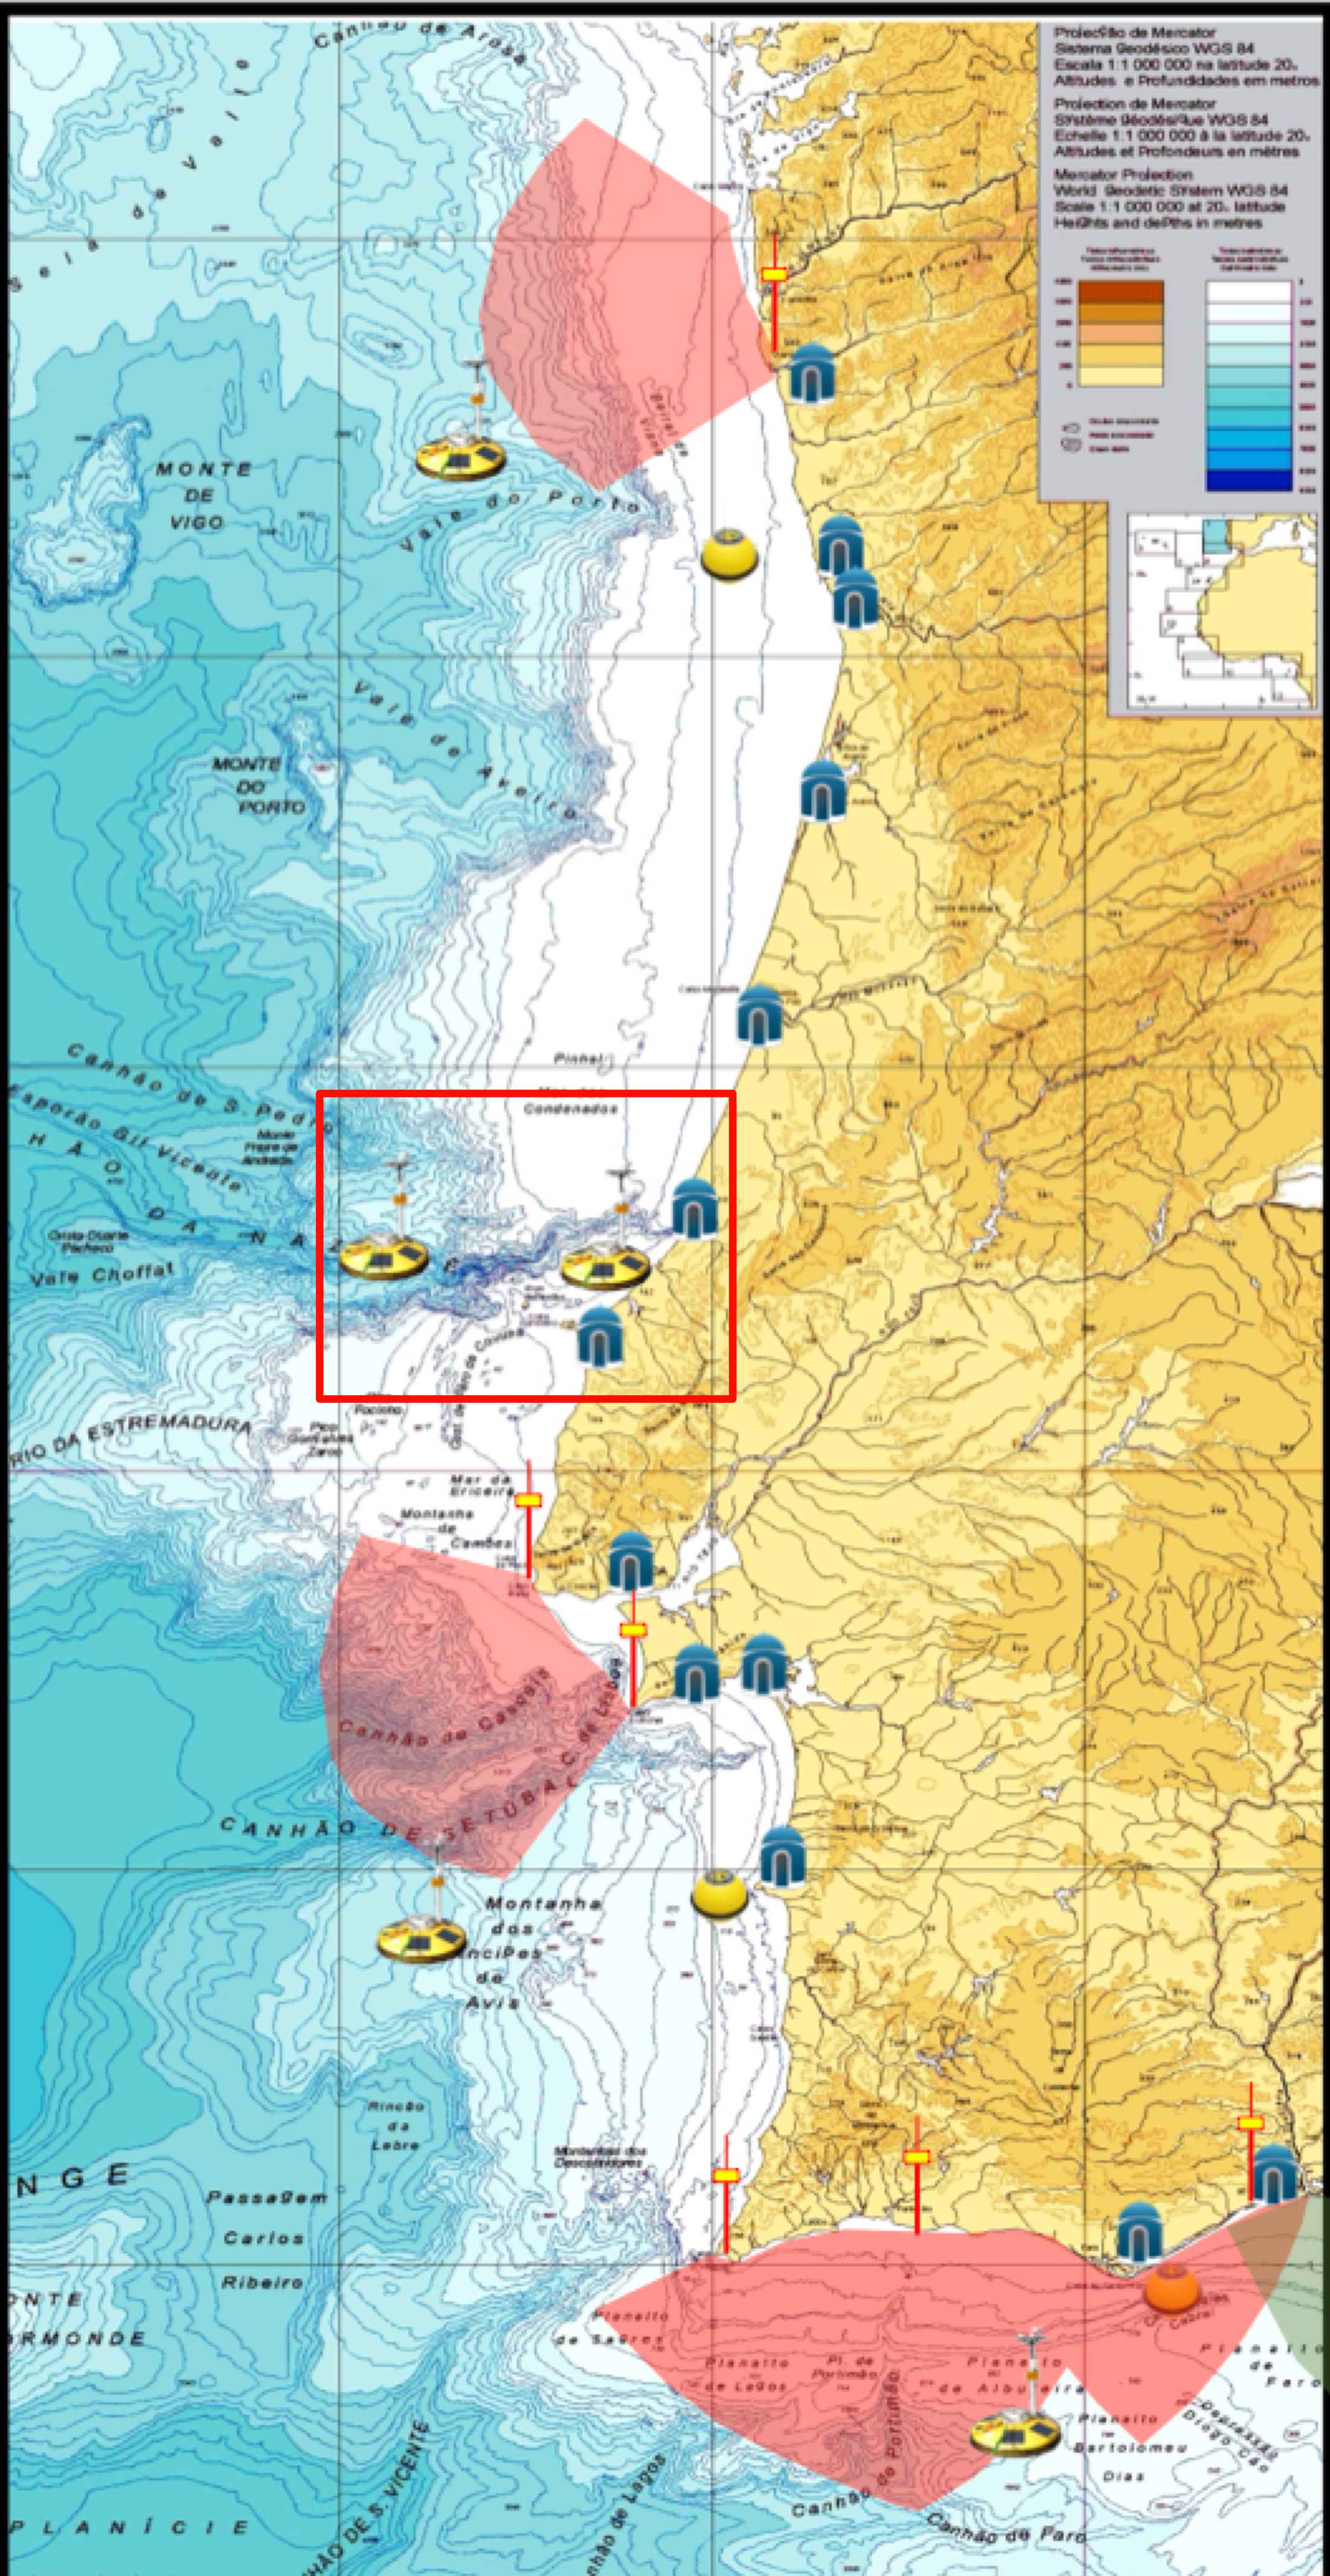
\includegraphics[scale=0.2]{fig/po-map.png}}
  \hspace{+0.3cm}
  \subfigure[Bathymetry showing the \naz canyon-Berlengas area
  and its environment.]{\label{fig:domain}\includegraphics[scale=0.19]{fig/area_ripples.png}}
  \caption{\subref{fig:po-map} \& \subref{fig:domain} show detailed
    views of the study area for \proj off the coast of mainland
    Portugal. The \naz Canyon is a significant feature of this area
    and a driver for the bio-geophysics of the domain
    \cite{tyler2009europe}.\kcomment{The white bands are shipping lanes?}}
  \label{fig:studyarea-1}
\end{figure}


In this study, we address the challenge of loop closure by
implementing and evaluating a complete data cycle — from model
prediction, to uncertainty projection, to adaptive sampling and data
assimilation. The work was conducted within the framework of \proj
(\textbf{F}ield expe\textbf{R}iments for mod\textbf{E}ling,
a\textbf{S}similatio\textbf{N} and adaptiv\textbf{E}
samp\textbf{L}ing), specifically designed to explore and test
model-driven robotic exploration strategies. % The experimental results
% obtained within the experiment serve to illustrate and validate the
% proposed approach, highlighting the practical benefits and challenges
% of real-world adaptive ocean exploration.

The study was conducted in the coastal ocean off central Portugal,
focusing on the region influenced by the \naz Canyon (39.2$^{\circ}$ -
39.9$^{\circ}$N) (Fig. \ref{fig:studyarea-1}) during fall of
2024. While the experiment considered the measurable impact of
model-driven robotic sampling to both the bio-geochemistry of the
canyon region, this manuscript is focused on the implications of
closing the \emph{sample-assimilate-predict-direct} loop closure.
% (Fig. \ref{fig:loop-closure}).

Implementing such a closed-loop system in a dynamic coastal
environment presents substantial challenges. These included the need
for high-resolution numerical models capable of rapidly generating
uncertainty projections, robust algorithms for exploration under a
range of constraints, reliable communication links for mission
updates, and assimilation frameworks that integrate heterogeneous
real-time data streams. Furthermore, marine operations face logistical
risks and communication limitations — such as low bandwidth,
intermittent connectivity, and unpredictable weather — that further
constrain the execution of adaptive sampling missions.

The \naz area features pronounced topographic contrasts: the
transition from the wide Estremadura Plateau to the narrower northern
shelf, the long and narrow \naz submarine canyon that incises the
shelf and extends more than 200km offshore, and the Berlengas
archipelago, a UNESCO Biosphere Reserve with high ecological
value. These features contribute to enhanced biological productivity
and biodiversity, and strongly modulate physical and biogeochemical
processes in the region.

Freshwater inputs from major rivers, such as the Tagus, have only a
limited direct impact on the area. In contrast, smaller rivers and the
\'{O}bidos lagoon can episodically deliver low-salinity, nutrient-rich
plumes to the shelf. Circulation is driven by seasonal wind
forcing linked with the Azores High, with persistent
upwelling-favorable northerly winds in summer and frequent downwelling
episodes in winter under southerly winds. The interplay between canyon
topography, shelf circulation, and atmospheric forcing generates
complex mesoscale dynamics, intensified tidal currents, and internal
wave activity that promote strong vertical mixing and cross-shelf
exchanges \cite{martins10,quaresma07}.

The combination of sharp bathymetric gradients, variable forcing, and
rich physical–biogeochemical interactions makes the \naz Canyon region
an ideal natural laboratory to test sampling strategies % . In
% particular, its dynamic environment posed both opportunities and
% challenges for the experiment, providing a representative coastal
% setting in which to
and evaluate how model-based uncertainty projections can guide
sampling and assimilation to improve ocean model predictive skill.


\proj itself is part of a larger concept for multi-domain sensing,
observation and exploration, which couples ocean models, autonomous
robotics, Artificial Intelligence and Machine Learning coupled with a
small satellite constellation \cite{rajan21}. Our end goal is to
democratize ocean model prediction by lowering costs, providing access
to a range of stakeholders, by integrating methods in low-cost
computation of modeling services coupled with spatio-temporal data
assimilation from mobile or immobile robots across space, aerial,
surface and underwater domains. 